\documentclass[english,11pt]{beamer}

\DeclareMathOperator{\Cov}{Cov}
\DeclareMathOperator{\Var}{Var}
\DeclareMathOperator{\E}{\mathbb{E}}
\DeclareMathOperator{\Proba}{\mathbb{P}}

\newcommand{\Covb}[2]{\ensuremath{\Cov\!\left[#1,#2\right]}}
\newcommand{\Eb}[1]{\ensuremath{\E\!\left[#1\right]}}
\newcommand{\Pb}[1]{\ensuremath{\Proba\!\left[#1\right]}}
\newcommand{\Varb}[1]{\ensuremath{\Var\!\left[#1\right]}}

% norm
\newcommand{\norm}[1]{\| #1 \|}

\newcommand{\indep}{\rotatebox[origin=c]{90}{$\models$}}





\usepackage{mathptmx,amsmath,amssymb,graphicx,bibentry,bbm,babel,ragged2e}

\makeatletter

\newcommand{\noun}[1]{\textsc{#1}}
\newcommand{\jitem}[1]{\item \begin{justify} #1 \end{justify} \vfill{}}
\newcommand{\sframe}[2]{\frame{\frametitle{#1} #2}}

\newenvironment{centercolumns}{\begin{columns}[c]}{\end{columns}}
%\newenvironment{jitem}{\begin{justify}\begin{itemize}}{\end{itemize}\end{justify}}

\usetheme{Warsaw}
\setbeamertemplate{footline}[text line]{}
\setbeamertemplate{headline}{}
\setbeamercolor{structure}{fg=purple!50!blue, bg=purple!50!blue}

\setbeamersize{text margin left=15pt,text margin right=15pt}

\setbeamercovered{transparent}


\@ifundefined{showcaptionsetup}{}{%
 \PassOptionsToPackage{caption=false}{subfig}}
\usepackage{subfig}

\usepackage[utf8]{inputenc}
\usepackage[T1]{fontenc}

\usepackage{multirow}

\usepackage{mdframed}


\makeatother

\begin{document}



\title{Construction of geo-commons by communities of practice: the case of orienteering maps generation from open LIDAR data}

\author{J.~Raimbault$^{1,2,3,4}$\\
\texttt{juste.raimbault@ign.fr}
}


\institute{$^{1}$LASTIG, Univ. Gustave Eiffel, IGN-ENSG\\
$^{2}$CASA, UCL\\
$^{3}$UPS CNRS 3611 ISC-PIF\\
$^{4}$UMR CNRS 8504 G{\'e}ographie-cit{\'e}s
}


\date{\textit{Journ{\'e}e de la Recherche UGE-IGN-ENSG 2024}\\
28/03/2023
}



%One important aspect of geo-commons lies in the diversity of their sourcing, and consequently in the possibility of crowdsourcing by domain experts in very specific contexts, enabled by the open sourcing of raw data, tools and methods. We propose in this contribution to illustrate such processes of geo-commons construction through the niche domain of orienteering maps generation from open LIDAR data. Forest orienteering maps have a large scale (1/10000 for middle distance and 1/15000 for long distance) and a quasi exhaustive description of topographic details, implying a very high production cost by expert cartographers. Although the interpretation and selection part remains crucial and fieldwork still necessary, base map automatic generation from LIDAR data has shown a significant potential in reducing mapping costs and times, but also in empowering runners to train on previsouly unmapped terrains. The free software Karttapullautin has allowed communities of practice of orienteering mappers in several countries (Norway, Finland, Switzerland, France, Spain, New Zealand) to systematically generate maps accross an unprecendeted coverage. We detail the different production contexts, in which institutional or private partners can be involved. Future work will include interviews with stakeholders in the various country contexts, to better understand stakes at play during the contruction of geo-commons.


\frame{\maketitle}

\sframe{Digital twins as commons?}{

More general framework of ``\textit{g{\'e}o-communs}'', launched by IGN since January 2021 \url{https://www.ign.fr/institut/la-demarche-geocommuns}.

\smallskip

\begin{center}

\includegraphics[width=0.15\linewidth]{figures/LOGO_IGN.png}
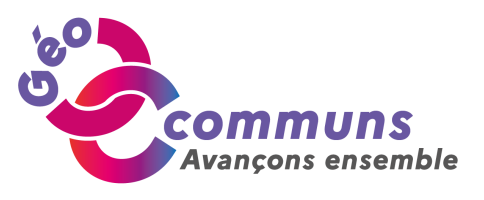
\includegraphics[width=0.54\linewidth]{figures/geocommuns.png}
\end{center}

\smallskip

$\rightarrow$ all IGN data is now open data 

$\rightarrow$ mutualisation, collaboration around tools, methods, databases

$\rightarrow$ public consultation in May 2021 (165 stakeholders from various backgrounds)

\medskip

\footnotesize

\textbf{Definition: } ``\textit{Geographic Information databases co-producted or co-maintained, and co-developped tools and methods, following an open common governance, to garantee a full appropriation by communities of users/producers/stakeholders/citizens}''

}

\sframe{Open questions for geocommons}{

\begin{enumerate}
	\item Governance of geocommons: mediator $\neq$ technical coordinator
	\item Economic model: public service (open public good)
	\item Core data: static digital twin at the national scale?
	\item Data production: e.g. link with OSM
	\item Licence: open licence but not ODbL?
	\item Methods and tools: ecosystem of open source softwares
	\item Open science as a part of geocommons
	\item Crucial role for environmental data
	\item Link with European directives for open data; European geocommons?
\end{enumerate}

}


\sframe{Research question}{


% ! def community of practice


}


\sframe{Orienteering maps}{

}

\sframe{Map generation from LIDAR data}{



}

\sframe{The Mapant initiative}{


% mention across Norway


}


\sframe{Comparative analysis}{

% institutional context

% licence: data, generated maps

% coverage

% usage?

}


\sframe{Future work}{

}


\sframe{Conclusion}{

}



%%%%%%%%%%%%%%%%%%%%%
\begin{frame}[allowframebreaks]
\frametitle{References}
\bibliographystyle{apalike}
\bibliography{biblio}
\end{frame}
%%%%%%%%%%%%%%%%%%%%%%%%%%%%






\end{document}










% slides last year


\sframe{Digital twins and sustainability: literature mapping}{

% si possible carto lit dig twin - sdgs

% Request : "digital twin" AND "sustainable development" (adding "sustainb*" -> too general, include sust economically e.g.)
%   initial corpus?

\justify

\textit{How do the two main themes of the conference go along in the literature?}

\medskip

\textit{What principal fields of study applying digital twins to sustainable development?}


\bigskip
\bigskip

$\rightarrow$ Using the methods and tools of \cite{raimbault2019exploration} \cite{raimbault2021empowering}, we do a systematic literature mapping using citation networks, constructed from google scholar data.

\medskip

$\rightarrow$ Starting from a seed corpus of 100 papers obtained with the request\\
\texttt{"digital twin" AND "sustainable development"}, we retrieve backward citations at depth two, to obtain a corpus of \textbf{14042 papers} with \textbf{24229 citation links}.

\medskip

$\rightarrow$ We analyse the citation network using community detection, to retrieve endogenous research fields.


}

\sframe{Main research areas from the literature mapping}{

\begin{columns}
	\begin{column}{0.6\linewidth}
		\includegraphics[width=1.1\linewidth]{figures/core_zoom}
	\end{column}
	\begin{column}{0.39\linewidth}
		\footnotesize
		\begin{itemize}
		    \item ``Smart manufacturing'' (21.9\%)
			\item Epistemology of DT (14.6\%)
			\item Civil engineering/BIM (11.4\%)
			\item Supply chain (6.8\%)
			\item Circular economy (5.6\%)
			\item Energy systems (5.1\%)
			\item Urban analytics/smart cities (5.0\%)
			\item ``Metaverse'' (4.5\%)
			\item ``Industry 4.0'' (4.2\%)
			\item ``Smart farming'' (4.0\%)
		\end{itemize}
	\end{column}
\end{columns}



}





\sframe{Digital twins: concepts and reality}{

\justify

% dig twins \cite{batty2018digital}

\textbf{Definition of a DT?} Coined in the 2000s from engineering \cite{batty2018digital}

\medskip

{\footnotesize ``\textit{A digital twin is a mirror image of a physical process [\ldots], usually matching exactly the operation of the physical process which takes place in real time.}''}

\medskip

$\rightarrow$ in practice not identical (example for cities: real-time GIS \cite{li2020real}); often not in real time or even dynamical.

\bigskip

The \textbf{link between the model (twin) and the system} is complex: which level of detail, which modelling choices, how to handle the resulting hybrid cyber-physical system? \cite{batty2019map}

``{\footnotesize \textit{A map is not the territory, or is it?}}''
% (inspire houllebeq et Levy) (meaning of representation)

\bigskip

% link with complexity \cite{arcaute2021future}

DT approaches too close to systems engineering, and often miss \textbf{social science/complexity} issues \cite{arcaute2021future}

$\rightarrow$ models at all time scales decision-making in the anthropocene.


}



\sframe{From digital twins to multiple simulation models}{


\justify

\textit{How to link digital twins and decision-making for sustainable development?}

\bigskip
\bigskip

$\rightarrow$ smart cities are on the long run: urban analytics for policy \\
\cite{kandt2021smart}

\bigskip

$\rightarrow$ unpredictability, multi-dimensionality, multi-scalarity of territorial systems: need for multiple models \cite{batty2021multiple}, multiple perspectives\\
 \cite{pumain2020conclusion}

\bigskip

$\rightarrow$ simulation models of territories for sustainable policies\\
\cite{raimbault2020empowering}


}









\sframe{Model integration: land-use transport interactions}{


\includegraphics[width=0.39\linewidth]{figures/accessp_withbridge_prd_EN.png}
\includegraphics[width=0.6\textwidth]{figures/macrocoevol_en.png}

\medskip


\textit{A modeling approach to the issue of structuring effects of transport infrastructures: co-evolution of networks and territories as a strong model integration}

\bigskip

\tiny
%\textcolor{grey}
Raimbault, J. (2019). Evolving accessibility landscapes: mutations of transportation networks in China. In Aveline-Dubach, N., ed. \textit{Pathways of sustainable urban development across China - the cases of Hangzhou, Datong and Zhuhai}, pp 89-108. Imago. ISBN:978-88-94384-71-0

\nocite{raimbault:halshs-02265423}

\smallskip

Raimbault, J. (2020). Indirect evidence of network effects in a system of cities. Environment and Planning B: Urban Analytics and City Science, 47(1), 138-155.

\nocite{raimbault2020indirect}

\smallskip

Raimbault, J. (2021). Modeling the co-evolution of cities and networks. In Handbook of Cities and Networks. Edward Elgar Publishing.

\nocite{raimbault2021modeling}


}


\sframe{Implementing horizontal model integration}{

\justify

\textit{Constructing a multimodal four step transport models by linking open components and data with scientific workflow engines}

\bigskip

\textbf{Integrated models:}

\begin{itemize}
	\item MATSim model (MATSim Community) for transport \cite{w2016multi}
	\item SPENSER model (University of Leeds) for synthetic population \cite{spooner2021dynamic}
	\item QUANT model (CASA, University College London) for spatial interactions \cite{batty2021new}
	\item spatialdata library (OpenMOLE community) for data processing \cite{raimbault2020scala}
\end{itemize}

\smallskip

\tiny

Raimbault, J., \& Batty, M. (2021). Estimating public transport congestion in UK urban areas with open transport models. GISRUK 2021 Proceedings.

\nocite{raimbault2021estimating}

}


\sframe{Model coupling: urban design and UHI}{

\begin{columns}
	\begin{column}{0.6\linewidth}
		\begin{center}
			\includegraphics[width=\linewidth]{figures/buildings_6.png}	
		\end{center}
	\end{column}
	\begin{column}{0.39\linewidth}
		\justify
		\textbf{SURe project} (collaboration LASTIG, ISC-PIF, EPIDAPO)
		
		\bigskip
		
		$\rightarrow$ coupling the SimPLU3D urban generative model \cite{brasebin2017apports} with an Urban Heat Island model to find compromises between density and the UHI effect. 

	\end{column}
\end{columns}




}


















